\chapter{Implementacija i korisničko sučelje}
		\section{Korištene tehnologije i alati}		
			 U tijeku razvoja projekta "Ozdravi", pažljivo su odabrane i implementirane različite tehnologije i alati kako bi se postigla efikasna izrada dokumentacije i aplikacije za zdravstveni sustav.
			 Za unapređenje timskih komunikacija korištene su aplikacije \textit{WhatsApp}\footnote{\url{https://www.whatsapp.com}} i \textit{Microsoft Teams}\footnote{\url{https://www.microsoft.com/en-us/microsoft-teams/group-chat-software}}. WhatsApp, popularna platforma za brzu razmjenu poruka, olakšala je neposrednu interakciju među članovima tima, dok je Microsoft Teams pružio šire mogućnosti za suradnju, uključujući organizaciju sastanaka, održavanje sastanaka i dijeljenje datoteka.
			 U praćenju zadataka i upravljanju projektom koristila se \textit{Jira}\footnote{\url{https://www.atlassian.com/software/jira}}, snažan alat koji je omogućio stvaranje strukturirane i pregledne radne okoline. Jira je poslužila kao središnje mjesto za praćenje i planiranje aktivnosti, olakšavajući koordinaciju među članovima tima.
			 \textit{GitHub}\footnote{\url{https://github.com}} se istaknuo kao ključni alat za upravljanje izvornim kodom i omogućavanje učinkovite suradnje među članovima tima. GitHub, kao web-bazirana platforma, pružio je mogućnost distribuiranog upravljanja verzijama korištenjem Git sustava. Repozitorij na GitHubu služio je kao centralno mjesto za čitav izvorni kod, omogućavajući članovima tima sinkroniziranje svojih lokalnih kopija koda, praćenje promjena te učinkovito upravljanje raznim granama razvoja.
			 \textit{Astah}\footnote{\url{http://astah.net/editions/professional}} je korišten za izradu UML dijagrama, pružajući jasan prikaz strukture sustava i odnosa između njegovih dijelova. Osim Astaha, korišteni su i drugi alati za izradu dijagrama, uključujući \textit{Visual Paradigm}\footnote{\url{https://online.visual-paradigm.com}} i \textit{Lucidchart}\footnote{\url{https://www.lucidchart.com}}.
			 Za razvoj frontend dijela aplikacije korišten je \textit{React}\footnote{\url{https://reactjs.org/}}, jedna od najpopularnijih \textit{JavaScript}\footnote{\url{https://www.javascript.com/}} biblioteka koja omogućava dinamičko i responzivno korisničko sučelje. React je pridonosio brzoj izgradnji modernog sučelja s visokom interaktivnošću.
			 Korišten je i \textit{Bootstrap}\footnote{\url{https://getbootstrap.com}}, popularni okvir za izradu responzivnih web stranica, koji je omogućio brzo i jednostavno oblikovanje sučelja te moderan i funkcionalan dizajn. Bootstrap pruža jednostavne i učinkovite klase za organizaciju elemenata, responzivno oblikovanje pomoću tzv. grid sustava te unaprijed definirane stilove za tipografiju, forme, gumbiće i mnoge druge komponente.
			 Za backend je odabran \textit{Spring}\footnote{\url{https://spring.io}}, robustan okvir za razvoj \textit{Java}\footnote{\url{https://www.java.com/en/}} aplikacija. Spring je pružio strukturu i podršku za izradu pouzdanih, sigurnih i skalabilnih backend rješenja.
			 API sustav je strukturiran i dokumentiran korištenjem alata \textit{Swagger}\footnote{\url{https://swagger.io}}, pri čemu je implementiran sukladno OpenAPI konvencijama. OpenAPI pristup omogućava jednostavno definiranje, dokumentiranje i testiranje RESTful API-ja te definiranje svih dostupnih endpointa, parametara, odgovora i modela podataka.
			 U procesu pisanja koda korišteni su \textit{IntelliJ IDEA}\footnote{\url{https://www.jetbrains.com/idea/}} i \textit{Visual Studio Code}\footnote{\url{https://visualstudio.microsoft.com/}}. IntelliJ IDEA, s bogatim skupom značajki, podržavao je razvoj Java aplikacija, dok je Visual Studio Code, lagan i svestran, omogućavao efikasno pisanje koda u različitim jezicima, uključujući \textit{JavaScript}\footnote{\url{https://www.javascript.com/}}.
			 Odabir ovih alata bio je prepušten osobnim preferencijama članova tima.
			 Za postavljanje produkcijskog okruženja odabran je Heroku kao infrastrukturna platforma. \textit{Heroku}\footnote{\url{https://www.heroku.com}} pruža stabilnost i skalabilnost, čineći implementaciju i održavanje aplikacije jednostavnim i učinkovitim.
			 Baza podataka \textit{PostgreSQL}\footnote{\url{https://www.postgresql.org}} koristila se za trajno pohranjivanje podataka. PostgreSQL je open-source sustav za upravljanje bazama podataka koji pruža pouzdano i sigurno okruženje za pohranu informacija.
			 U konačnici, ovom kombinacijom tehnologija postignuto je stvaranje moderne zdravstvene aplikacije koja je intuitivna za korisnike, prilagodljiva potrebama zdravstvenog sustava i unapređuje ukupno iskustvo krajnjih korisnika.
			\eject 
	
		\section{Ispitivanje programskog rješenja}
			Ispitivanje programskog rješenja predstavlja ključan korak u procesu razvoja programske podrške s ciljem ostvarivanja nekoliko ključnih prednosti:
			\begin{packed_item}
				\item olakšava dodavanje značajki - ispitivanje osigurava da nove promjene ne narušavaju funkcionalnost postojećeg koda
				\item sprječava unošenje grešaka u kod - kvalitetni testovi detektiraju neispravan kod prije nego što postane dio projekta čime se smanjuje mogućnost pojave grešaka
			\end{packed_item}
			
			U sklopu ovog projekta koristili smo dvije vrste ispitivanja:
			\begin{packed_item}
				\item Ispitivanje komponenti (eng. Unit Testing)
				\item Ispitivanje sustava (eng. Integration Testing)
			\end{packed_item}
			
			
			Ispitivanjem komponenti koristeći JUnit biblioteke osigurali smo ispravan rad ključnih dijelovi backenda. Ispitivanjem sustava provjerili smo ispravnost povezanosti backenda i frontenda iz perspektive krajnjeg korisnika.
			Ispitivanje sustava je provedeno koristeći Selenium biblioteke.
			
			%==========================================================================================================================%
			\subsection{Ispitivanje komponenti}
			\subsubsection*{Test 1: Ispitivanje ispravnog OIB-a}
			Komponenta: ValidityUtil \newline
			Metoda: public static boolean isValidOib(String oib); \newline
			Ulazni Podaci: 
			\begin{packed_item}
				\item String oib : "39751670659"
			\end{packed_item}
			Očekivani rezultat:
			\begin{packed_item}
				\item Metoda vraća istinu (true) jer je OIB ispravan prema standardu za OIB-e.
			\end{packed_item}
			\lstinputlisting[style=JavaStyle, caption={Test 1}]{code/oib_test_1.java}

			\subsubsection*{Test 2: Ispitivanje neispravnog OIB-a}
			Komponenta: ValidityUtil \newline
			Metoda: public static boolean isValidOib(String oib); \newline
			Ulazni Podaci: 
			\begin{packed_item}
				\item String oib : "397516706.9"
			\end{packed_item}
			Očekivani rezultat:
			\begin{packed_item}
				\item Metoda vraća laž (false) jer OIB sadrži '.', odnosno ne zadovoljava standardni oblik.
			\end{packed_item}
			\lstinputlisting[style=JavaStyle, caption={Test 2}]{code/oib_test_2.java}

			U testovima namijenjenima testiranju kontrolera, želimo ispitati isključivo ponašanje kontrolera, bez ispitivanja servisa, baze i drugih dijelova aplikacije.
			Budući da kontroleri ne mogu raditi bez tih dijelova, nužno je stvoriti "mock" objekte koji ih mijenjaju i simuliraju njihovo ponašanje.

			Ovaj postupak uključuje ručno stvaranje entiteta koji predstavljaju očekivane rezultate servisa.

			\subsubsection*{Test 3: Dohvaćanje popisa Uputa.}
			Komponenta: InstructionsController \newline
			Zahtjev: HTTP GET /instructions \newline
			Mock Podaci:
			\begin{packed_item}
				\item Korisnik
				\item Pregledi kojima korisnik može pristupiti
			\end{packed_item}
			Očekivani rezultat:
			\begin{packed_item}
				\item Kontroler u JSON formatu vraća popis svih Uputa koje trenutni korisnik može vidjeti, HTTP odgovor ima status 201 (OK).
			\end{packed_item}
			\lstinputlisting[style=JavaStyle, caption={Test 3}]{code/instruction_test_1.java}
			
			\subsubsection*{Test 4: Stvaranje Uputa.}
			Komponenta: InstructionsController \newline
			Zahtjev: HTTP POST /instructions \newline
			Mock Podaci:
			\begin{packed_item}
				\item Korisnik (ADMIN)
			\end{packed_item}
			Očekivani rezultat:
			\begin{packed_item}
				\item Kontroler u JSON formatu vraća atribute novostvorene Upute, HTTP odgovor ima status 201 (Created).
			\end{packed_item}
			\lstinputlisting[style=JavaStyle, caption={Test 4}]{code/instruction_test_2.java}

			\subsubsection*{Test 5: Dohvaćanje nepostojeće Upute.}
			Komponenta: InstructionsController \newline
			Zahtjev: HTTP GET /instruction/\{id\} \newline
			Mock Podaci:
			\begin{packed_item}
				\item Korisnik (ADMIN)
			\end{packed_item}
			Očekivani rezultat:
			\begin{packed_item}
				\item HTTP odgovor ima status 404 (Not Found).
			\end{packed_item}
			\lstinputlisting[style=JavaStyle, caption={Test 5}]{code/instruction_test_3.java}

			\subsubsection*{Test 6: Dohvaćanje svih doktora u aplikaciji.}
			Komponenta: UsersController \newline
			Zahtjev: HTTP GET /users/doctors \newline
			Mock Podaci:
			\begin{packed_item}
				\item Korisnik (PARENT)
			\end{packed_item}
			Očekivani rezultat:
			\begin{packed_item}
				\item HTTP odgovor ima status 403 (Forbidden), jer roditelj ne smije dobiti popis svih liječnika u aplikaciji.
			\end{packed_item}
			\lstinputlisting[style=JavaStyle, caption={Test 6}]{code/user_test_1.java}
			
			\subsubsection*{Test 7: Dodavanje korisnika.}
			Komponenta: UsersController \newline
			Zahtjev: HTTP POST /users \newline
			Mock Podaci:
			\begin{packed_item}
				\item Korisnik (ADMIN)
			\end{packed_item}
			Očekivani rezultat:
			\begin{packed_item}
				\item Kontroler u JSON formatu vraća atribute novostvorenog Korisnika, HTTP odgovor ima status 201 (Created).
			\end{packed_item}
			\lstinputlisting[style=JavaStyle, caption={Test 7}]{code/user_test_2.java}

			\subsubsection*{Test 8: Registracija korisnika.}
			Komponenta: AuthenticationController \newline
			Zahtjev: HTTP POST /register \newline
			Očekivani rezultat:
			\begin{packed_item}
				\item Kontroler u JSON formatu vraća atribute novostvorenog Korisnika, HTTP odgovor ima status 201 (Created).
			\end{packed_item}
			\lstinputlisting[style=JavaStyle, caption={Test 8}]{code/registration_test.java}

			\begin{figure}[H]
				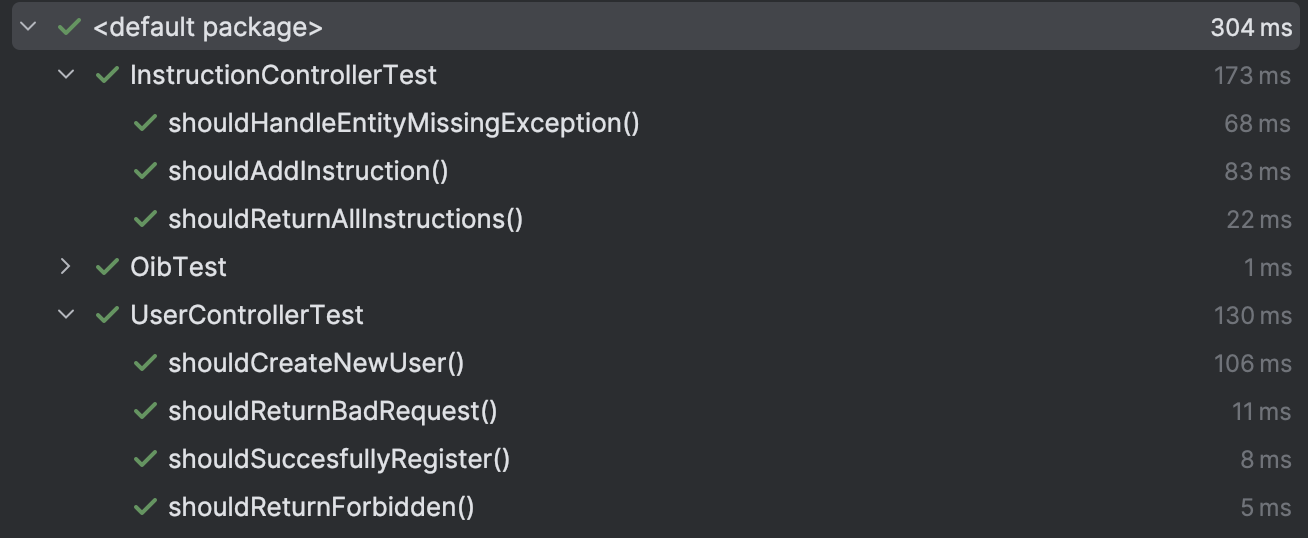
\includegraphics[width=\textwidth]{slike/testing_results.png} 
				\caption{Rezultati testiranja na lokalnom stroju.} 
			\end{figure}
			
			%==========================================================================================================================%
			\subsection{Ispitivanje sustava}
			Testovi ispitivanja sustava su napisani u Selenium IDE dodatku za preglednik i prate nekoliko obrazaca uporabe, ali su vezani uz jednu cjelinu - rad s preporukama za bolovanje.
			U ovom scenariju testiranja sudjeluje više uloga (roditelj, pedijatar, liječnik) i svi koraci koje jedna uloga izvodi su grupirani u zasebnu grupu koraka. Također, za svaki korak je
			naveden i pripadajući očekivani rezultat.
			
			 \subsubsection*{Grupa koraka 1: Dodavanje preporuke za bolovanje}
			 Koraci:
			 \begin{packed_enum}
				\item Prijava u sustav kao pedijatar ("pedijatar@mail.com")
				\item Odabir opcije "Bolovanja" iz alatne trake.
				\item Odabir opcije "Dodaj preporuku"
				\item Odabir pregleda na temelju kojeg se izdaje preporuka ("Tamara Stanic 2023-12-25") unutar modalnog ekrana.
				\item Odabir opcije "Spremi".
			 \end{packed_enum}
			 Očekivani rezultati:
			 \begin{packed_enum}
				\item Pedijatar se može prijaviti u sustav.
				\item Postoji opcija "Bolovanja" u alatnoj traci.
				\item Dostupna je opcija "Dodaj preporuku".
				\item Postoji izbornik pregleda unutar modalnog ekrana u kojem je moguće izabrati traženi pregled.
				\item Postoji opcija "Spremi" unutar modalnog ekrana.
			 \end{packed_enum}
			 
			 \begin{figure}[H]
				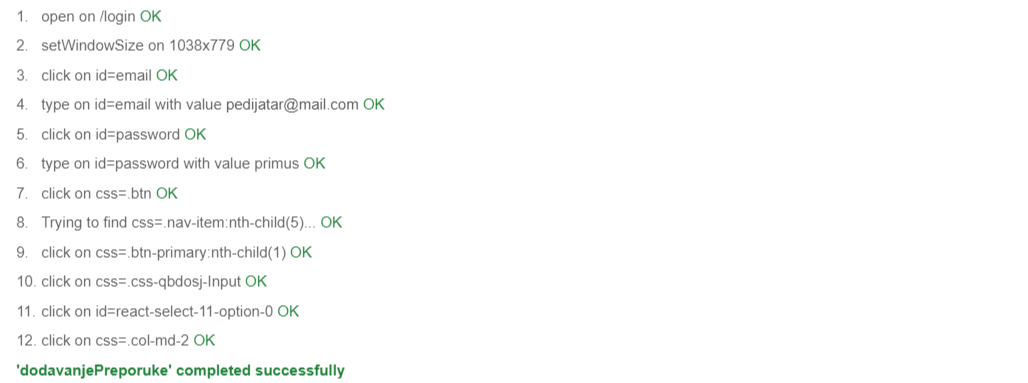
\includegraphics[width=\textwidth]{slike/selenium1.1.png} 
				\caption{Rezultati testiranja grupe koraka 1} 
			\end{figure}

			\begin{figure}[H]
				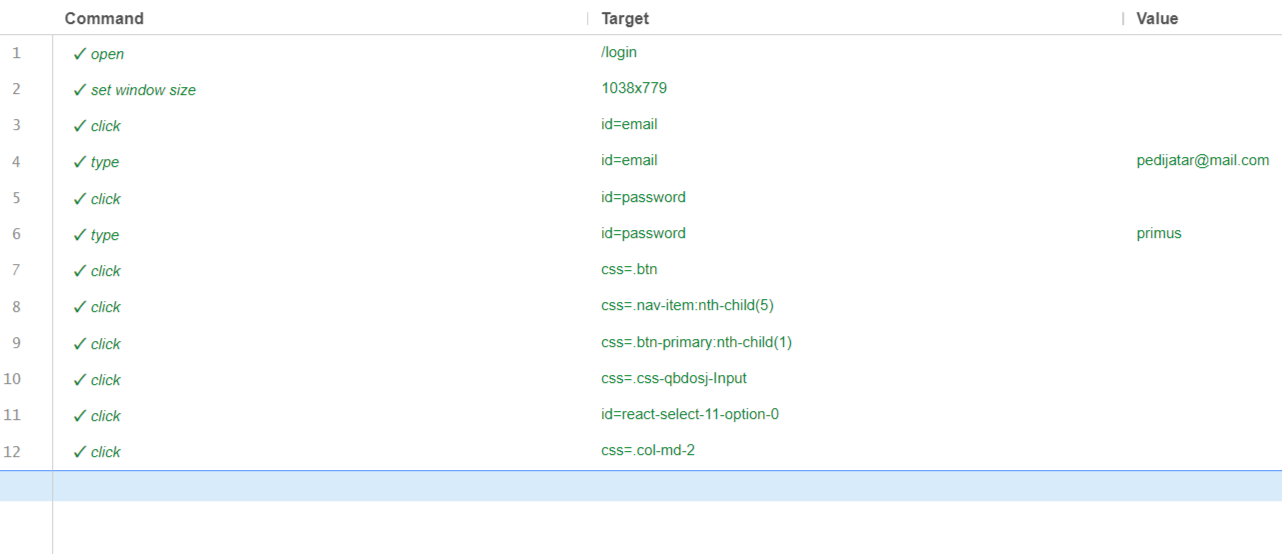
\includegraphics[width=\textwidth]{slike/selenium1.2.png} 
				\caption{Rezultati testiranja grupe koraka 1} 
			\end{figure}

			 \subsubsection*{Grupa koraka 2: Pregled neobrađene preporuke za bolovanje}
			 Koraci:
			 \begin{packed_enum}
				\item Prijava u sustav kao roditelj ("roditelj@mail.com")
				\item Odabir opcije "Bolovanja" iz alatne trake.
				\item Odabir preporuke iz popisa preporuke ("Tamara Stanic 2023-12-25").
			 \end{packed_enum}
			 Očekivani rezultati:
			 \begin{packed_enum}
				\item Roditelj se može prijaviti u sustav.
				\item Postoji opcija "Bolovanja" u alatnoj traci.
				\item Postoji tražena preporuka za bolovanje u popisu preporuka.
				\item Pod "Status" piše "Čeka odobrenje." unutar modalnog ekrana.
			 \end{packed_enum}

			 
			 \begin{figure}[H]
				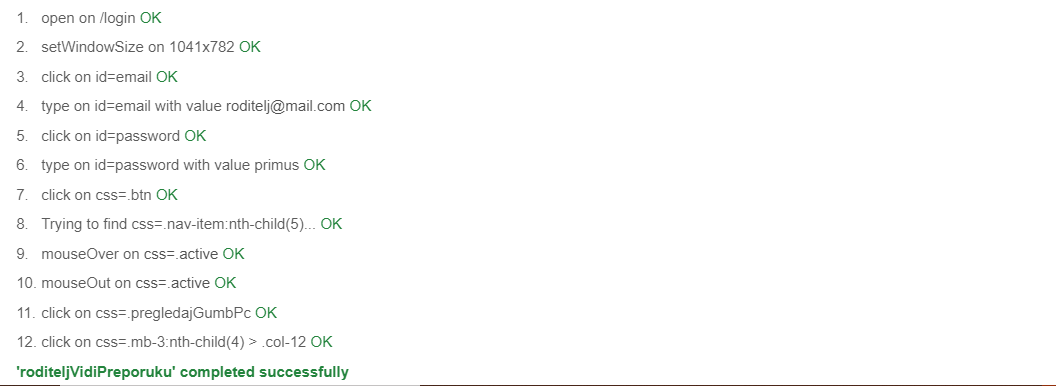
\includegraphics[width=\textwidth]{slike/selenium2.1.png} 
				\caption{Rezultati testiranja grupe koraka 2} 
			\end{figure}

			\begin{figure}[H]
				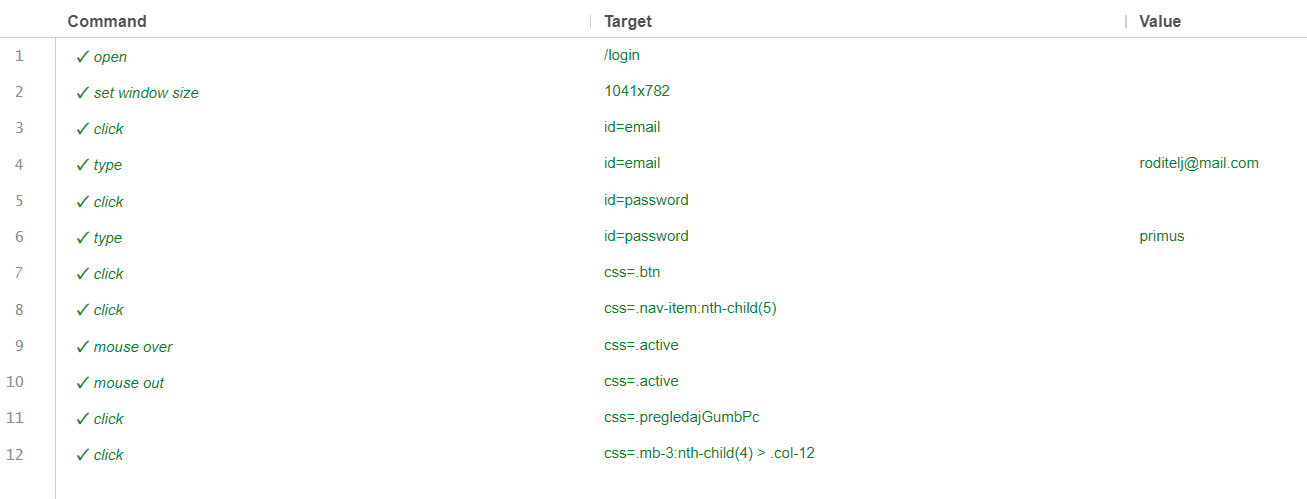
\includegraphics[width=\textwidth]{slike/selenium2.2.png} 
				\caption{Rezultati testiranja grupe koraka 2} 
			\end{figure}

			 \subsubsection*{Grupa koraka 3: Odobravanje preporuke za bolovanje}
			 Koraci:
			 \begin{packed_enum}
				\item Prijava u sustav kao liječnik obiteljske medicine ("doktor@mail.com")
				\item Odabir opcije "Bolovanja" iz alatne trake.
				\item Odabir preporuke iz popisa preporuke ("Tamara Stanic 2023-12-25").
				\item Odabir opcije "Odobri" iz modalnog ekrana.
			 \end{packed_enum}
			 Očekivani rezultati:
			 \begin{packed_enum}
				\item Liječnik obiteljske medicine se može prijaviti u sustav.
				\item Postoji opcija "Bolovanja" u alatnoj traci.
				\item Postoji tražena preporuka za bolovanje u popisu preporuka.
				\item Postoji opcija "Odobri" unutar modalnog okvira.
			 \end{packed_enum}

			 \begin{figure}[H]
				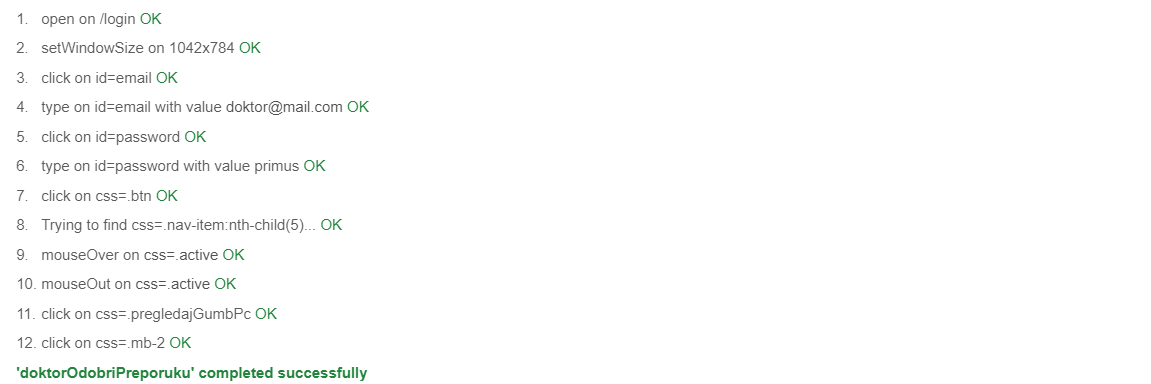
\includegraphics[width=\textwidth]{slike/selenium3.1.png} 
				\caption{Rezultati testiranja grupe koraka 3} 
			\end{figure}

			\begin{figure}[H]
				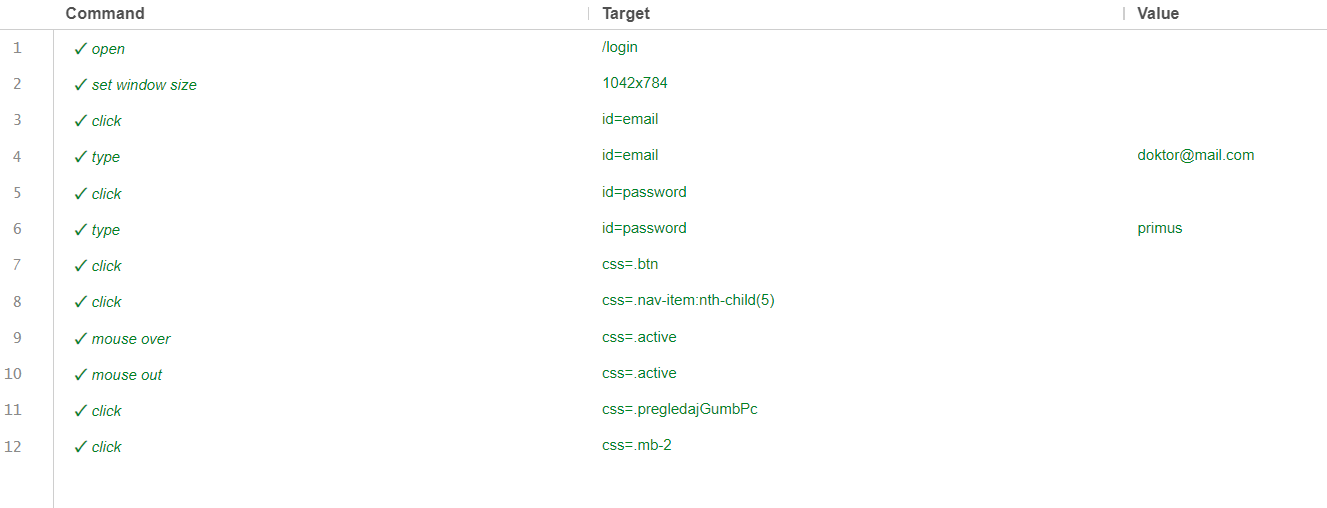
\includegraphics[width=\textwidth]{slike/selenium3.2.png} 
				\caption{Rezultati testiranja grupe koraka 3} 
			\end{figure}

			 \subsubsection*{Grupa koraka 4: Pregled odobrene preporuke za bolovanje}
			 Koraci:
			 \begin{packed_enum}
				\item Prijava u sustav kao roditelj ("roditelj@mail.com")
				\item Odabir opcije "Bolovanja" iz alatne trake.
				\item Odabir preporuke iz popisa preporuke ("Tamara Stanic 2023-12-25").
			 \end{packed_enum}
			 Očekivani rezultati:
			 \begin{packed_enum}
				\item Roditelj se može prijaviti u sustav.
				\item Postoji opcija "Bolovanja" u alatnoj traci.
				\item Postoji tražena preporuka za bolovanje u popisu preporuka.
				\item Pod "Status" piše "Odobreno." u modalnom ekranu preporuke.
			 \end{packed_enum}
			
			\begin{figure}[H]
				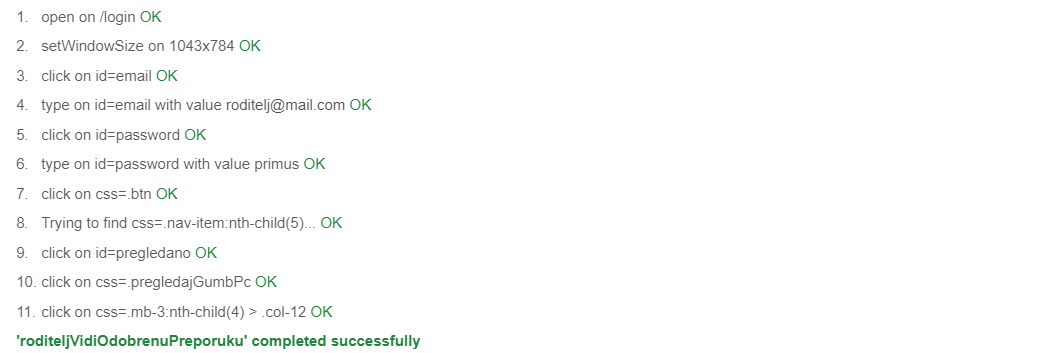
\includegraphics[width=\textwidth]{slike/selenium4.1.png} 
				\caption{Rezultati testiranja grupe koraka 4} 
			\end{figure}

			\begin{figure}[H]
				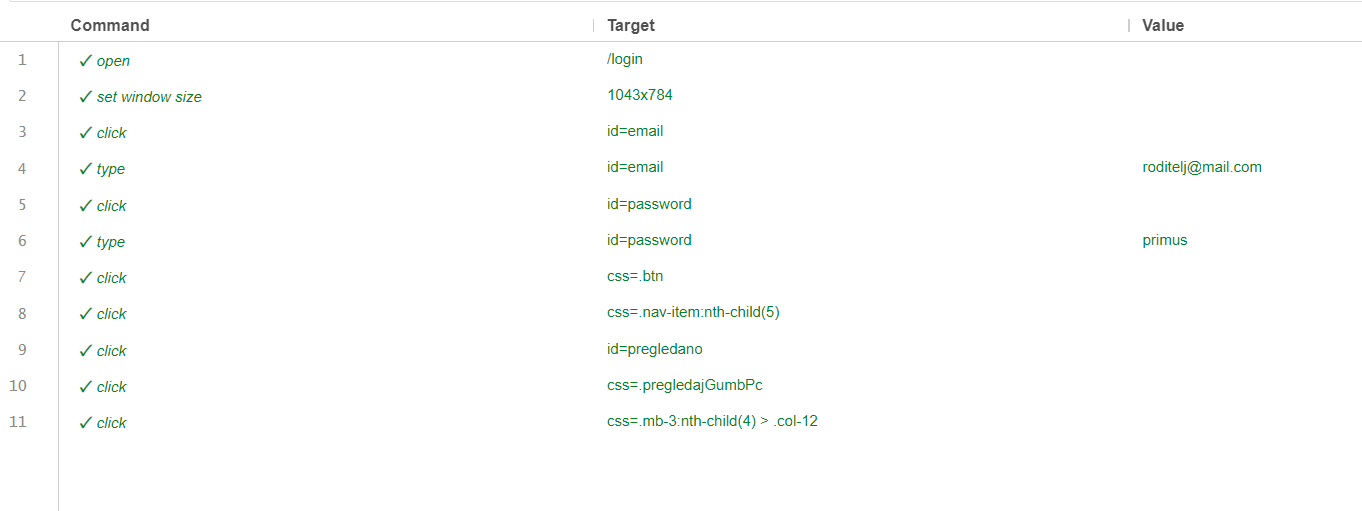
\includegraphics[width=\textwidth]{slike/selenium4.2.png} 
				\caption{Rezultati testiranja grupe koraka 4} 
			\end{figure}

			\eject
		
		\section{Dijagram razmještaja}
			Dijagrami razmještaja prikazuju konfiguraciju sklopovlja i programske podrške koja se koristi za implementaciju sustava u njegovom operativnom okruženju. Na cloud platformi smješten je poslužitelj baze podataka te web poslužitelji za backend i frontend. Korisnici pristupaju web aplikaciji putem svog web preglednika. Sustav je temeljen na arhitekturi "klijent - poslužitelj" s komunikacijom između korisničkih računala (roditelj, pedijatar, doktor, administrator) i poslužitelja putem HTTPS veze.
			\begin{figure}[H]
				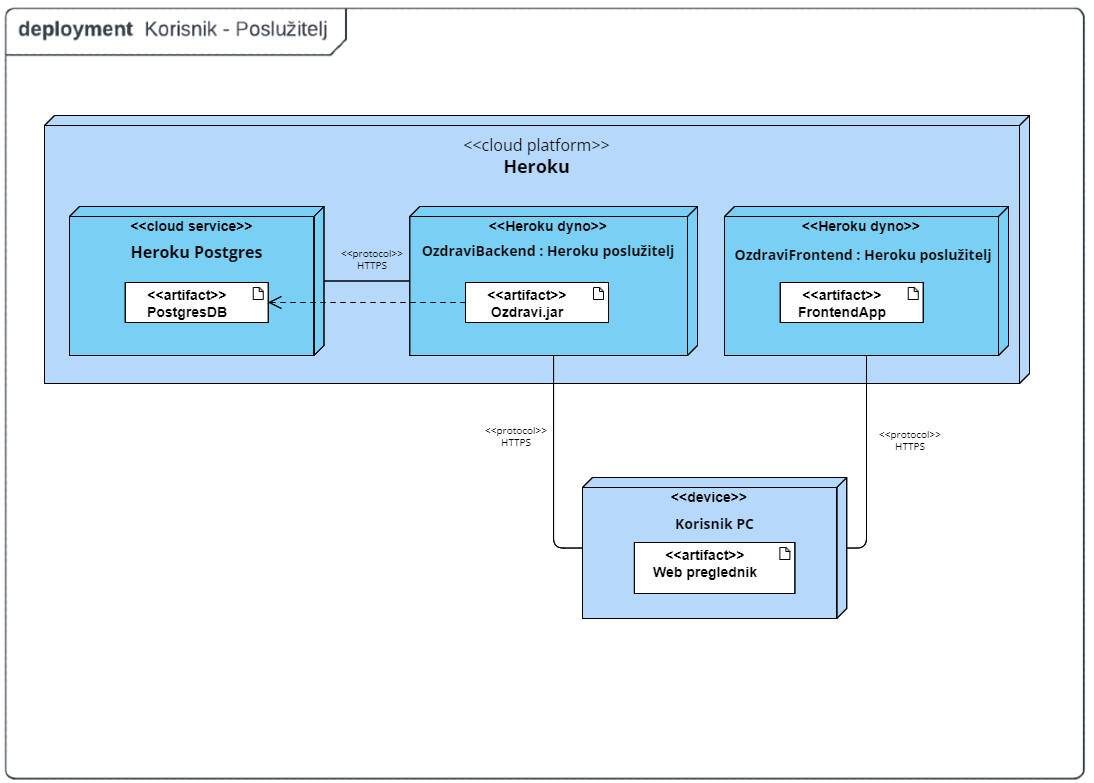
\includegraphics[width=\textwidth]{slike/deploymentDiagram.png} 
				\caption{Dijagram razmještaja} 
			\end{figure}
			\eject 
		
		\section{Upute za puštanje u pogon}
			Aplikacija "Ozdravi" se sastoji od nekoliko dijelova koje je potrebno postaviti kako bi se pokrenula u lokalnom okruženju.
		
			\subsection*{Postavljanje baze podataka}
			U procesu postavljanja baze podataka za aplikaciju "Ozdravi", prvi korak je instalacija relacijske baze podataka
			\href{https://www.postgresql.org/download/}{\textit{PostgreSQL-a}}. Nakon završetka instalacije, slijedi standardni postupak postavljanja korisničkog imena i lozinke (neobavezno).
			Nakon uspješne instalacije, potrebno je pristupiti konzoli baze (psql) kako bi se stvorili potrebni resursi za rad backenda aplikacije "Ozdravi".
	
			Nakon toga, izvršavaju se sljedeće naredbe:
			\lstinputlisting[style=SQLStyle, caption={Postavljanje baze podataka}]{code/db_setup.sql}

			Sada bi trebala biti stvorena baza podataka "ozdravi", čiji je vlasnik korisnik "welebyte". Naredbom \textit{\textbackslash l} može se provjeriti lista svih postojećih 
			baza podataka i njihovih vlasnika.
			\begin{figure}[H]
				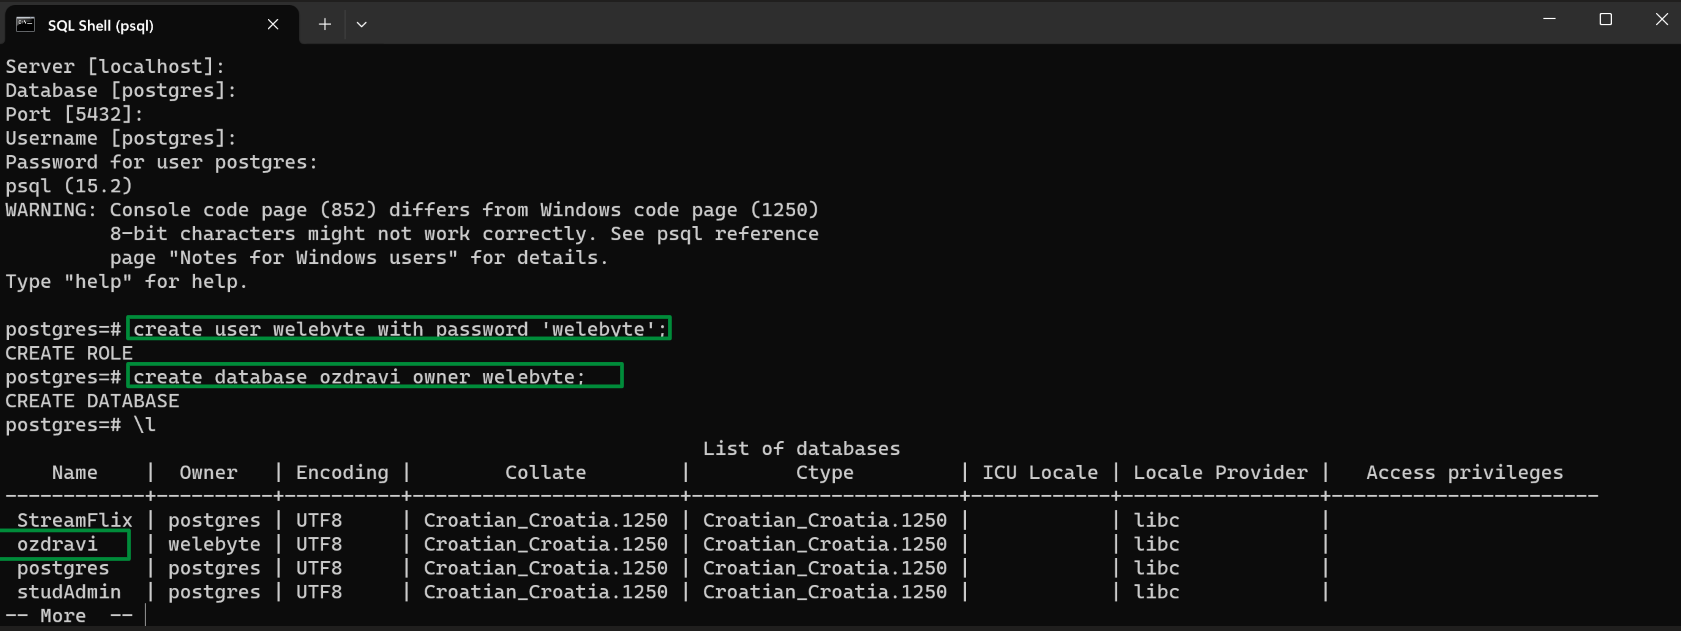
\includegraphics[width=\textwidth]{slike/sqlshell2.png} 
				\caption{Postavljanje baze podataka} 
			\end{figure}
	
			\subsection*{Postavljanje i pokretanje backenda aplikacije}
			Backend aplikacije je pisan u Javi 17, što znači da je na sustavu koji pokreće aplikaciju potrebno imati instaliran JDK (Java Development Kit) - preporučujemo \href{https://www.openjdk.org}{\textit{OpenJDK}} kao open-source implementaciju.
			Osim Jave, potrebno je imati i instaliran \href{https://maven.apache.org/download.cgi}{\textit{Apache Maven}}. To je alat koji koristimo za upravljanje bibliotekama i "buildovima" backend aplikacije.
			
			Pri pokretanju, potrebno je u konzoli otvoriti mapu \textit{IzvorniKod/ozdravi-backend}, a aplikacija se dalje kompajlira izvršavanjem sljedećih naredbi:
			\lstinputlisting[style=ShellStyle, caption={Instalacija i kompajliranje backenda}]{code/mvn_cmd.shell}

			te se pokreće izvršavanjem sljedeće naredbe: 
			\lstinputlisting[style=ShellStyle, caption={Pokretanje backenda}]{code/java_jar.shell}
			
			Aplikacija je sada dostupna na portu 8080 lokalnog stroja.

			\subsection*{Postavljanje frontenda}
			Frontend aplikacije pisan je u Reactu te za njegovo pakiranje i pokretanje je potrebno preuzeti \href{https://nodejs.org/en/download/}{Node.js}.

			Pri pokretanju, potrebno je u konzoli otvoriti mapu \textit{IzvorniKod/ozdravi-frontend} i izvršiti sljedeće naredbe:
			\lstinputlisting[style=ShellStyle, caption={Instalacija i pokretanje frontenda}]{code/npm_cmd.shell}

			Prvu je naredbu potrebno izvršiti samo jednom, kako bi se prikupili potrebni paketi, a druga je naredba pokreće server na kojem je frontend dostupan za preuzimanje.
			
			\newpage \noindent Nakon pokretanja, aplikaciju je moguće vidjeti na adresi: \url{http://localhost:3000.}\\
			\begin{figure}[H]
				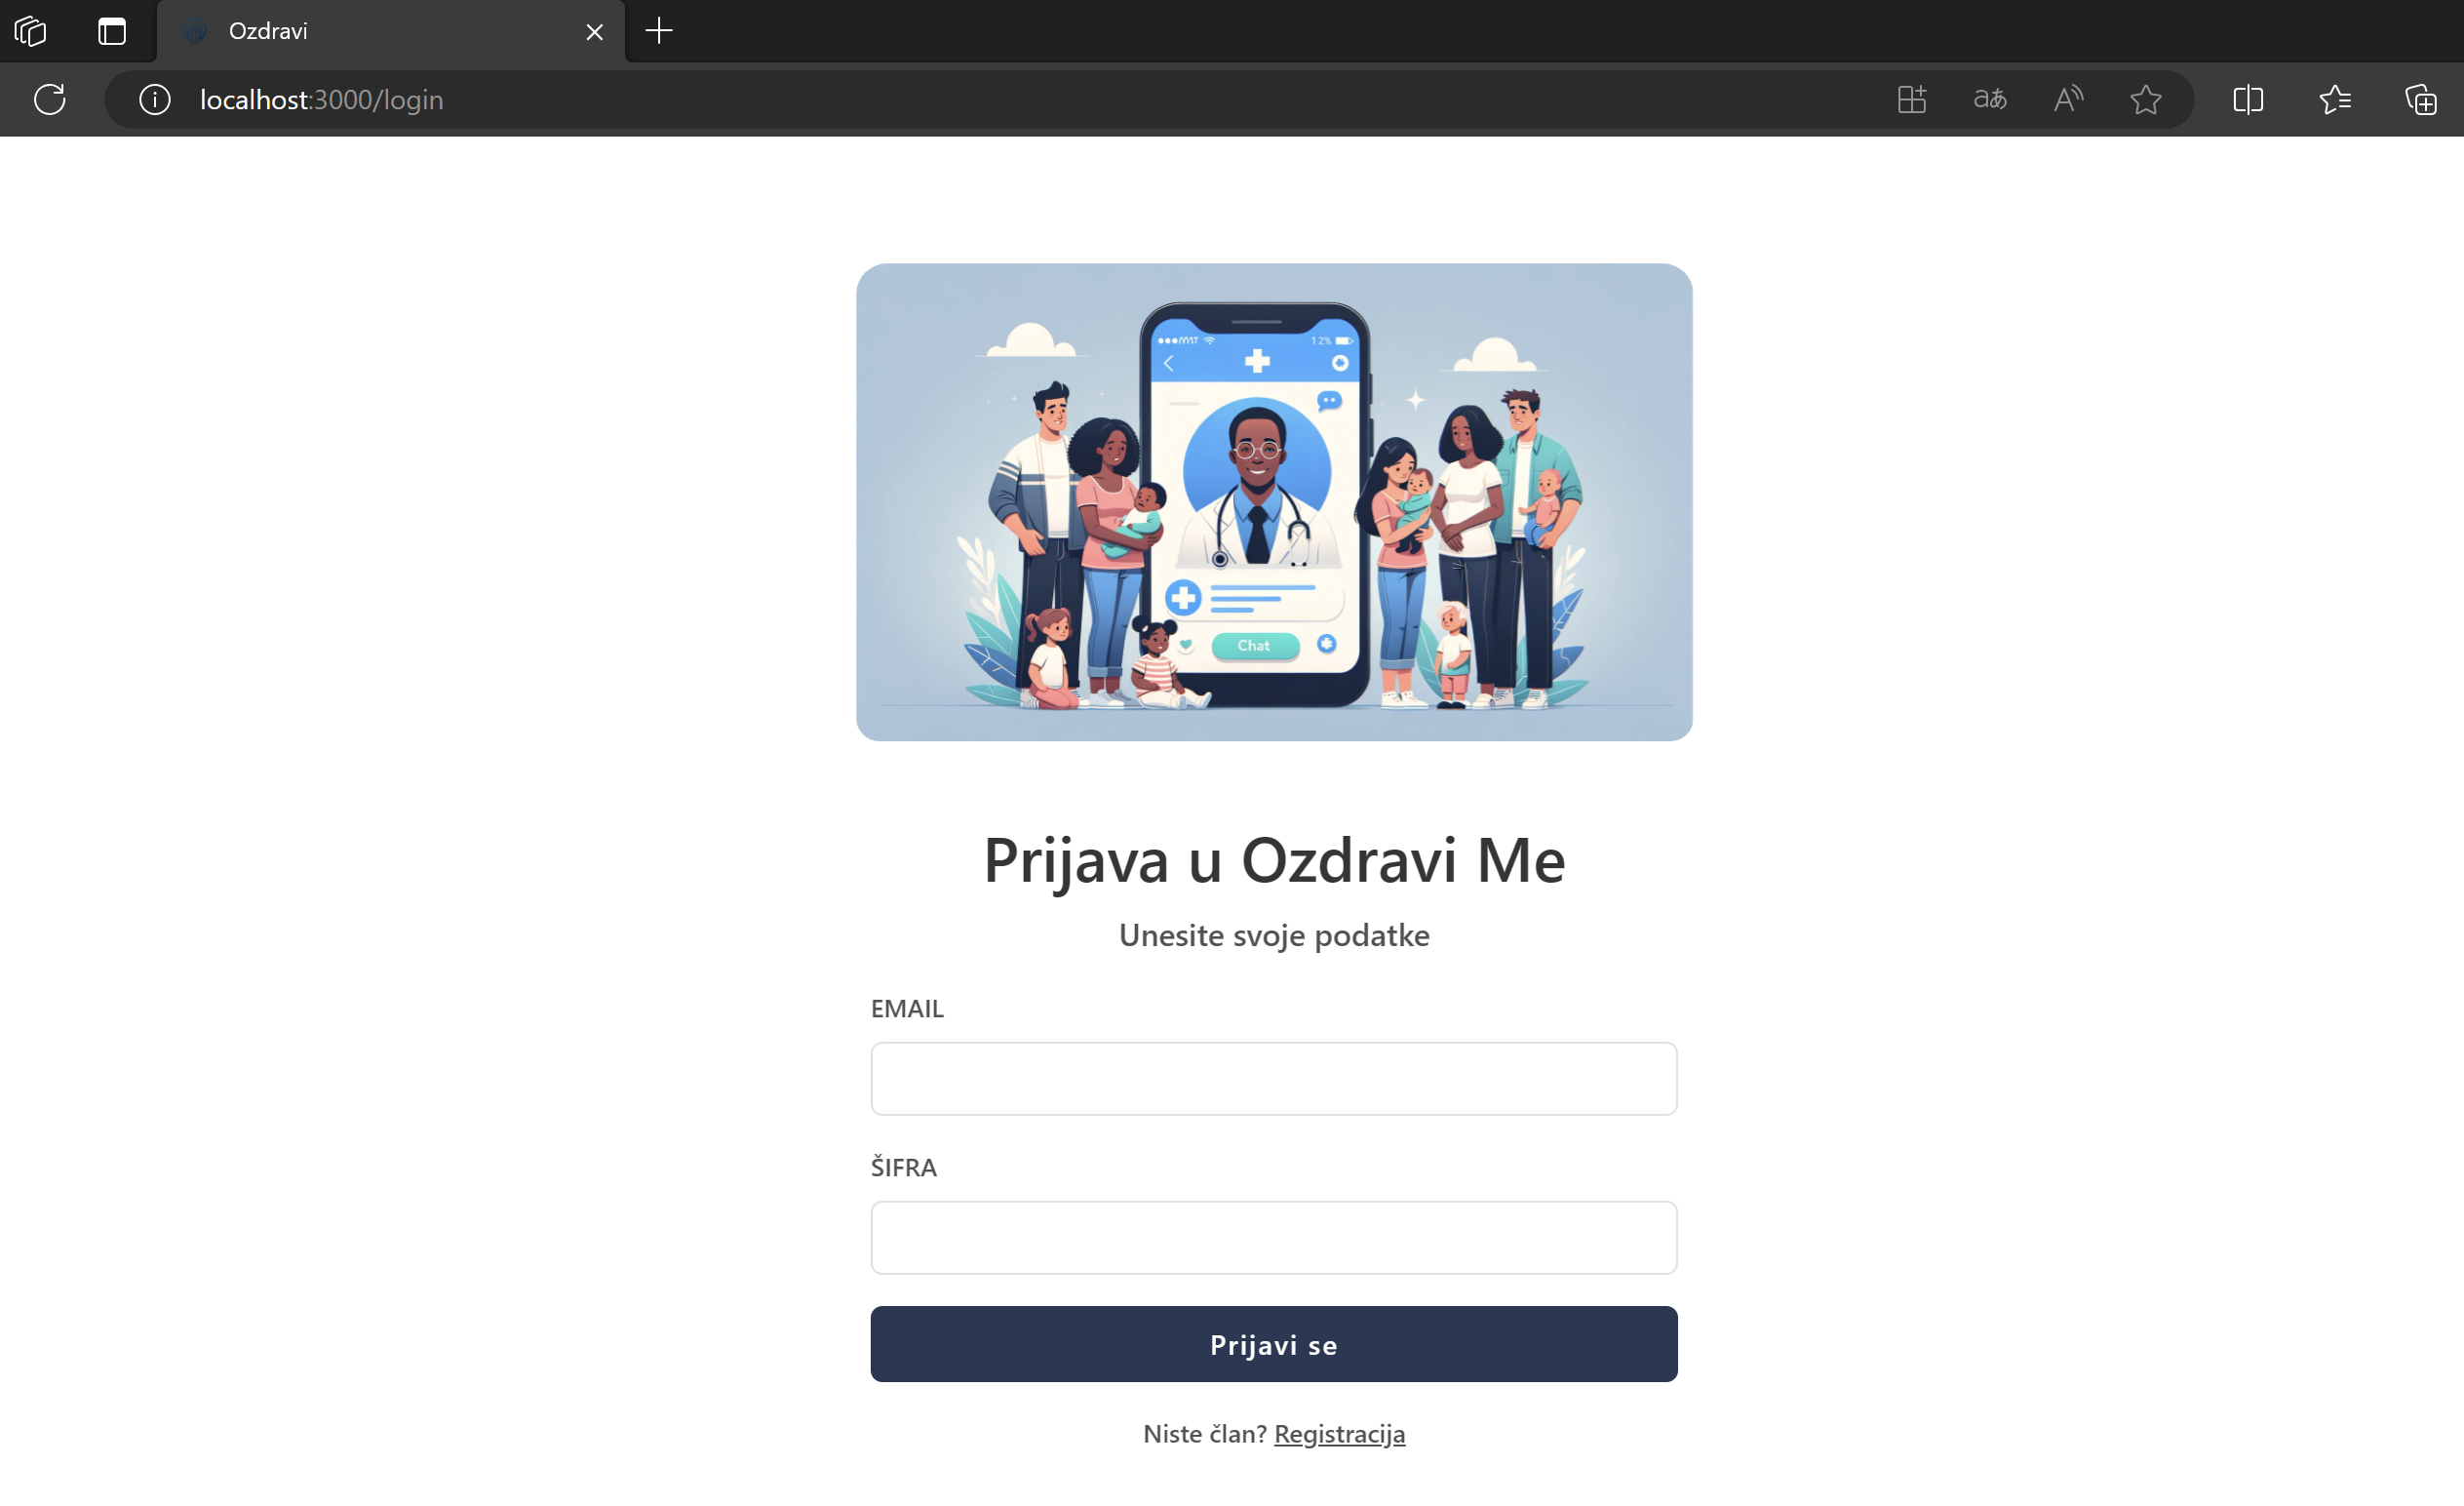
\includegraphics[width=\textwidth]{slike/loc3000.png} 
				\caption{Aplikacija na portu 3000} 
			\end{figure}
			Nakon svake promjene i spremanja koda, stranica se automatski ponovno učitava. Osim toga, postoji mogućnost promjene porta aplikacije uređivanjem datoteke \textit{package.json}, 
			gdje se u liniji koda \textit{"start": set PORT=3006 \&\& react-scripts start} može izmijeniti broj porta prema želji.
			
			\subsubsection*{Deployment nove verzije aplikacije}
			Svi dijelovi aplikacije se, u produkcijskom okruženju, pokreću na Heroku platformi. Za sam "build" aplikacije se koriste već gotovi "buildpackovi" za Javu, odnosno React koje osigurava Heroku.
			Naše Heroku okruženje je povezano s repozitorijem aplikacije na GitHubu i Heroku može preko "GitHub Deployments" povući izvorni kod i provesti proces isporuke.
			S obzirom da je cijela aplikacija sadržana u jednom repozitoriju, a sastoji se od dvaju dijelova koji se neovisno isporučuju, morali smo prilagoditi "build" proces tome. 

			Način na koji je infrastruktura aplikacije postavljena ne podržava automatsko pokretanje build procesa (npr. kad se pull request mergea) već je potrebno unutar sučelja Herokua ručno pokrenuti isporuku frontend, odnosno backend dijela aplikacije.
			\begin{figure}[H]
				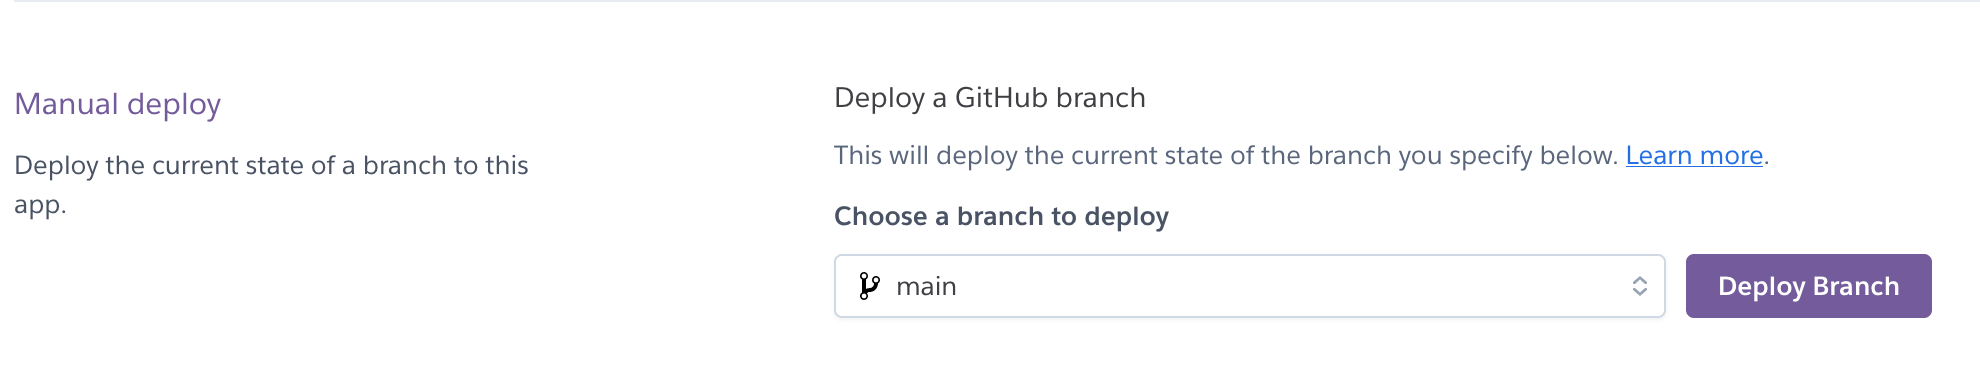
\includegraphics[width=\textwidth]{slike/heroku_interface.png} 
				\caption{Sučelje Heroku platforme} 
			\end{figure}
			
			\subsubsection*{Stvaranje PDF izvještaja dokumentacije}
			Dokumentacija za ovaj projekt je napisana koristeći paket \LaTeX  i nalazi se u mapi \textit{Dokumentacija/}. Kako bi se iz .tex datoteka izgradio PDF izvještaj potrebno je na računalu imati instalaciju \LaTeX-a i pokrenuti ispravne naredbe za izgradnju PDF-a (npr. \textit{latexmk}).
			\eject 